\begin{frame}
  \frametitle{Angle between line and plane}
     Line $L: \quad \textbf{r}= \textbf{r}_1+t\textbf{u}$ \hspace{2cm}
     Plane $\mathcal{P}: \quad (\textbf{r}-\textbf{r}_0) \cdot \textbf{n} = 0$

   \begin{columns}[t]
    \column[T]{6cm}
    %
    Line \textcolor[rgb]{0.98,0.00,0.00}{perpendicular} to plane\\
    \uncover<2->{
    $L \bot \mathcal{P}$ $\Longleftrightarrow$
    $\textbf{u} \| \textbf{n}$ $\Longleftrightarrow$ \\
    $$\boxed{\textbf{u} \times \textbf{n} = \textbf{0}}$$}
    %
    \uncover<3->{
    \textcolor[rgb]{0.98,0.00,0.00}{Angle} between line and plane\\
    %
    $\alpha$: angle between $L$, $\mathcal{P}$ $\Longleftrightarrow$ \\
    $\alpha$: acute angle $\textbf{u}$, $\textbf{\text{orth}}_{\bm{n}}\textbf{u}$} \uncover<4->{$\Longleftrightarrow$
    $$\boxed{\alpha = \arcsin\left( \frac{|\textbf{u} \cdot \textbf{n}|}{|\textbf{u}| \, |\textbf{n}|}\right) }$$}
    \uncover<5->{\textcolor[rgb]{0.98,0.00,0.00}{Intersection}:}
    \uncover<6->{$$(\textbf{r}_1+t\textbf{u}-\textbf{r}_0) \cdot \textbf{n} = 0$$
    $$(\textbf{r}_1-\textbf{r}_0)\cdot \textbf{n} + t \textbf{u} \cdot \textbf{n} = 0$$
    Solve for $t$.}
    \column{6.5cm}
    %
    \begin{figure}
        \psfrag{L}{$L$}
        \psfrag{cP}{$\mathcal{P}$}
        \psfrag{P0}{$P_0(\textbf{r}_0)$}
        \psfrag{P1}{$P_1(\textbf{r}_1)$}
        \psfrag{P2}{$P_2$}
        \psfrag{a}{$\alpha$}
        \psfrag{orth}{$\textbf{\text{orth}}_{\bm{n}}\textbf{u}$}
        \psfrag{u}{$\textbf{u}$}
        \psfrag{n}{$\textbf{n}$}
        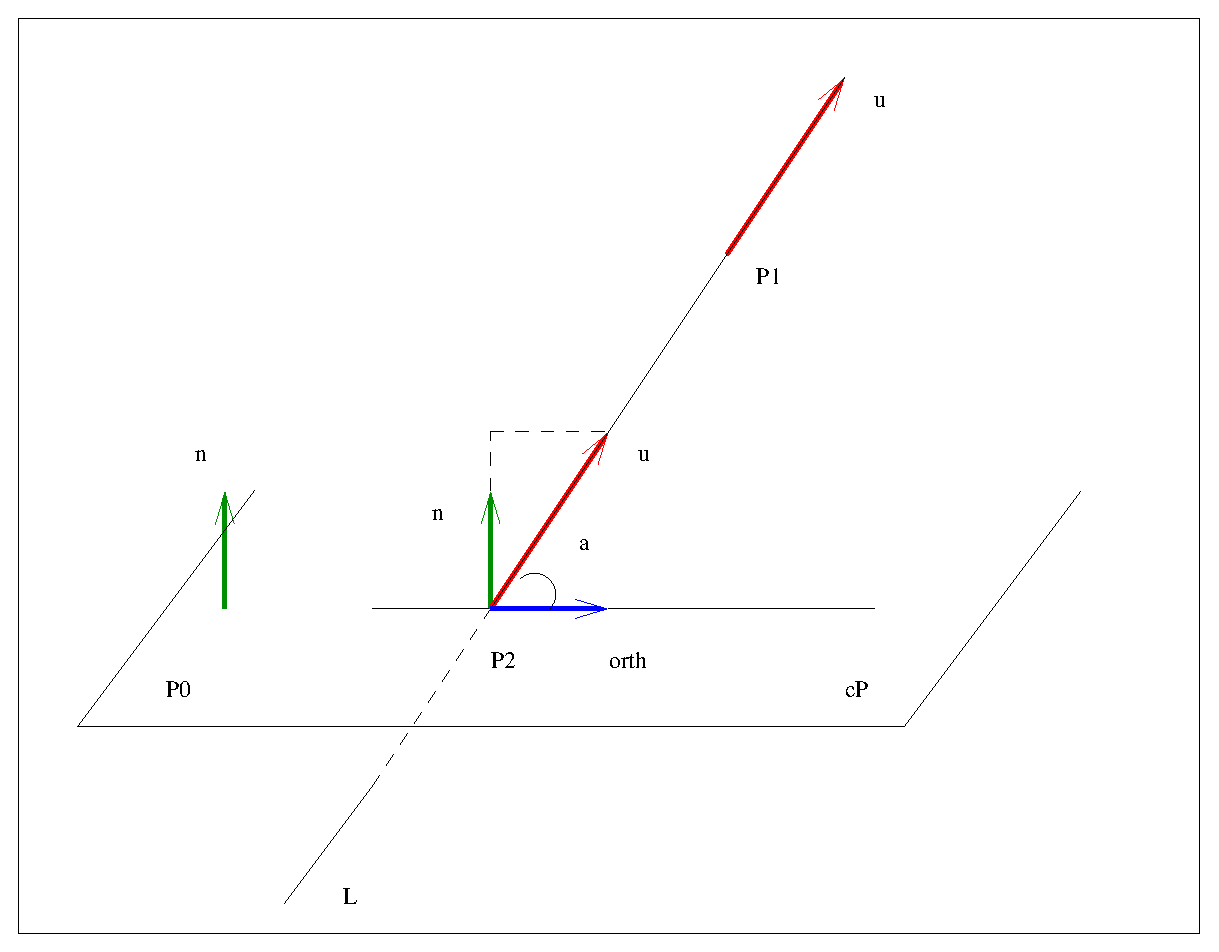
\includegraphics[height=2in]{../../modules/vectors/pictures/ok-angle_line_plane.eps}
    \end{figure}
  \end{columns}
\end{frame}